\documentclass{article}
\usepackage{graphicx}
\usepackage{amsmath}
\usepackage{amsfonts}
\usepackage[parfill]{parskip}
\usepackage{hyperref}
\usepackage[useregional]{datetime2}

\usepackage{biblatex}
\addbibresource{references.bib}

\usepackage[T1]{fontenc}
\usepackage{tgbonum}

\usepackage{listings}
\usepackage{xcolor}

\usepackage{longtable}

% Define a custom color
\definecolor{backcolour}{rgb}{0.95,0.95,0.92}
\definecolor{codegreen}{rgb}{0,0.6,0}

% Define a custom style
\lstdefinestyle{myStyle}{
    backgroundcolor=\color{backcolour},   
    commentstyle=\color{codegreen},
    basicstyle=\ttfamily\footnotesize,
    breakatwhitespace=false,         
    breaklines=true,                 
    keepspaces=true,                 
    numbers=left,       
    numbersep=5pt,                  
    showspaces=false,                
    showstringspaces=false,
    showtabs=false,                  
    tabsize=2,
}

% Use \lstset to make myStyle the global default
\lstset{style=myStyle}

\graphicspath{ {./figures/} }

% \title{CS-C3240: Machine Learning\\
%     \large Project report: Phishing Websites Detection
% }
% \author{Cuong Nguyen\\ \href{mailto:cuong.c.nguyen@aalto.fi}{cuong.c.nguyen@aalto.fi} }

\title{CS-C3240: Machine Learning\\
    \large Project report: Phishing Websites Detection}

\newcommand{\inlinemaketitle}{{\let\newpage\relax\maketitle}}


\begin{document}

\inlinemaketitle
% \tableofcontents
% \newpage

% \listoffigures
% \newpage

% Content of report would be written here
% \include{./tex/task1.tex}
% ...
% \include{./tex/task2.tex}

% \section{Introduction}
Phishing, a pervasive cybercrime, has significantly escalated its attacks on the
digital landscape.As an increasing number of users rely on online platforms for
banking, government services, and other critical activities, their sensitive
information, including identification numbers, usernames, passwords, and banking
credentials, is at risk of exposure to malicious actors. The ease with which
counterfeit websites can be created, mirroring the appearance and content of
legitimate ones, makes users particularly susceptible to inadvertently entering
their personal data into fraudulent domains. To mitigate this threat and safeguard
internet users from phishing attacks, a robust phishing detector or classifier is
essential. Leveraging the power of machine learning algorithms, the phishing detector
employed in this project effectively categorizes websites as either
\emph{Phishing} or \emph{Legitimate}.

The report is structured as the following: \autoref{sec:prob-formulation} formulates
the problem by introducting the data set, specifically labels and features.
\autoref{sec:method} explains feature selection and introduces chosen
machine learning models. \autoref{sec:result} shows the final results of
proposed models and compares the performance between different approaches.
\autoref{sec:conclusion} presents conclusions based on the results shown
in \autoref{sec:result}.
\section{Problem Formulation}\label{sec:prob-formulation}

% Subsection Dataset
\subsection{Dataset}
The Phishing Dataset
contains 5000 instances of phishing webpages and 5000 of legitimate webpages which
were collected from January to May 2015 and from May 2017 to June 2017~\cite{dataset-source}. By leveraging
the browser automation framework, Selenium WebDriver, extracted features are more
precise and robust compared to the regular-expression-based approaches~\cite{CHIEW2019153}.
All webpages in the dataset originates from the following sources:
\begin{itemize}
    \item Phishing webpage: PhishTank, OpenPhish
    \item Legitimate webpage: Alexa, Common Crawl
\end{itemize}

This dataset is WEKA-ready, which means that it is in a format compatible with the
WEKA\footnote{https://waikato.github.io/weka-wiki/} machine learning workbench.

% Subsection Label
\subsection{Label}
In this project, I will develop a machine learning (ML) model that could detect whether a given
website is a phishing or not. Each instance in the dataset is labeled as a phishing
or a legitimate webpage by a value of 1 or 0 respectively at the \emph{label} column.
In other words, the aim of this project is to develop a supervised machine learning model
to classify a given website into two classes, \emph{Phishing} and \emph{Legitimate}, based
on selected features obtained from the dataset.

\subsection{Feature}
There are 48 features in total, which most of them are the number of occurences of suspicious
HTML elements or characters in URL or in web context, which are discrete values. Besides, there are
continuous features which are the percentage of external hyperlinks, resources, redirects in the
HTML webpage source code. Moreover, there are binary features indicating True/False boolean
value as 1/0. For example:
\begin{itemize}
    \item \emph{DoubleSlashInPath}: Check if ``//'' exist in path of URL.
    \item \emph{NoHttps}: Check if HTTPS exist in URL.
\end{itemize}

Additionally, there are categorical features which are encoded into three integer values: -1,0,1.

A full list of features could be investigated at~\cite{CHIEW2019153}\footnote{See a summary of features
at~\autoref{tab:all_features}}.

\section{Methods}\label{sec:method}

% Subsection Feature Engineering
\subsection{Feature Engineering}
As there are in total 48 features corresponding to only 10000 data poinst, it has pitfalls
if the ML model is trained onto all features which number of them show weak correlationship to
the labels. Additionally, with the fixed number of training samples, the predictive
power of a ML model starts deteriorating when the number of dimensions, or features, exceeds
a certain dimensionality~\cite{problem-dimension}. Hence, keeping the number of features growing
does mean increasing the accuracy of predictions.

To decide which subset of features I should rely on, I took a reference on the baseline features
showed in~\cite{CHIEW2019153}. That baseline feature set were extracted by a feature selection
framework introduced in~\cite{CHIEW2019153}. Along with those 10 baseline features, I analyzed
the correlation coefficients between all features and label by utlizing Mutual Information (MI).
I selected MI since it measures the general dependence between variables, both linear and non-linear
relationship, which is unlike other common approaches such as Spearman or Pearson which only measure
the linear dependence~\cite{MI-score}.\autoref{fig:mi_score} shows MI scores of all 48 features
sorted in the ascending order. I selected top 15 features which have the highest MI score then did
union to the baseline feature subset to have the final feature sets for training. As a result,
I obtained a set of 16 features as shown in~\autoref{tab:feature_description}. The number of
features, or dimensions, is sufficient for the dataset of 10,000 entries and not too large leading
to the curse of dimensionality.


% Subsection Machine Learning Model
\subsection{Model}
\subsubsection{Logistic Regression}
In this supervised classification task, I selected Logistic Regression (LR) as a machine learning method since it
is a binary classification and easily interpretable. LR categorizes data points by feature vectors
$\mathbf{x} \in \mathbb{R}^n$ and binary lables $y$, $y \in \{0,1\}$ (encoded to \{Legitimate, Phishing\}) in this case.
The model uses a linear hypothesis $h(\mathbf{x}) = w^T\mathbf{x}$, with some parameter vector
$w \in \mathbb{R}^n$, to predict a binary label $y$~\cite{ml-book}.

I used the binary logistic loss function
\begin{align}
    L((\mathbf{x},y),h) = log(1+exp(-yh(\mathbf{x})))
\end{align}
where $x$ is feature vectors, $y$ is the true binary label (0 or 1), and $h$ is the linear hypothesis~\cite{ml-book}.
The reason behind this selection is that it is intuitive and already integrated into
\href{https://scikit-learn.org/stable/}{scikit-learn}.
Moreover, it penalizes incorrect predictions more heavily than correct predictions, which is suitable for
the aim of this task where I need to detect phishing websites.

\subsubsection{Random Forest}
As shown in~\cite{CHIEW2019153,SAHINGOZ2019345}, Random Forest (RF) outperforms other
classifier in phishing detection. Additionally, unlike LR, RF does not rely on the
linear relationship so that it is able to handle non-linear, more complex, relationships
between features. Those were two main logically reasons leaded me to choose RF as
a second machine learning model for this phishing dectection task. The loss function for
RF in classification is the impurity of individual decision region for labels~\cite{ml-book}.

Regarding the splitting criteria, loosely understood as a loss function for decision trees,
Gini impurity was selected due to its fast computation and good performance on balanced
data set. Gini impurity measures the heterogeneity of a node, quantifying how often
a randomly chosen element from the set would be incorrectly classified if it was labeled
according to the distribution of labels in that node. Mathematically, Gini impurity is
expressed:

\begin{align}
    I_G(p) = 1 - \sum_{i=1}^{K}p_i^2
\end{align}

where $K$ is the set of classes, $p_i$ is the probability of choosing an item with label
$i$~\cite{gini-formula}. The goal during training is to minimize the Gini impurity of
the resulting child nodes, creating more homogeneous groups.

\subsubsection{Model Evaluation}

To evaluate the models, I used \emph{Precision} score as the main benchmark during hyperparameter-tuning.
Additionally, in a phishing dectection context, it is also more important to dectect all
phishing pages, even if some legitimate pages are misclassified, so the \emph{Recall} metric was also
considered during hyperparameter-tuning. Hence, \emph{F1-Score } was also used to find balance
between \emph{Precision} and \emph{Recall} metrics.

% Subsection Training and Validation Dataset
\subsection{Training and Validation Set}
The dataset itself is balanced between two classes, 5000 data poitns for each class, so class balancing step
is no needed. Following the ``thumbs-up'' rule, I splitted the dataset into three sets, following the ratio 70/15/15,
into three subsets: training, validation, and testing. As a result, the training, validation, and testing subset
has 7000, 1500, and 1500 data points respectively. I chose this ratio of splitting as it is widely used and accepted
in the machine learning community. Moreover, this ``hold-out'' technique generates a sufficiently large size of
training and validation data. Importantly, dataset was shuffled to avoid biased sampling. Given three sets, I
fed the training set to the learning model, then evaluated it using the validation set. If the current parameter
and configuration of the hypothesis model has a good performance, I will do final testing and benchmark on the
testing set.
% \section{Results}\label{sec:result}
\subsection{Logistic Regression}
By running \href{https://scikit-learn.org/stable/modules/generated/sklearn.model_selection.GridSearchCV.html}{GridSearchCV} 
with the grid parameters (regularization strength, norm of the penalty, and optimization algorithm),
each with 5-fold cross-validation, I obtained the most optimal model with the following parameters:
inverse of regularization strength 10, L1 penalty, and \emph{liblinear} solver.

The optimal LR model generated the classification results shown in \autoref{tab:lr_val_report}:
\begin{table}[ht!]
    \centering
    \begin{tabular}{|c|c|c|c|}
        \hline
         & Precision & Recall & F1-Score \\
        \hline
        Legitimate (0) & 0.93 & 0.92 & 0.92 \\
        Phishing (1) & 0.92 & 0.93 & 0.93 \\
        \hline
        Accuracy & & & 0.92  \\
        \hline
    \end{tabular}
    \caption{Classification Report of the LR model on the validation set.}
    \label{tab:lr_val_report}
\end{table}

Generally, the LR had quite good performance on the validation set: all evaluation metrics
were greater than 0.9. Moreover, \emph{Recall} of the \emph{phishing} class was greater
than its \emph{Precision}, which satisfied the importance of misclassified phishing websites.

\subsection{Random Forest}
\href{https://scikit-learn.org/stable/modules/generated/sklearn.model_selection.GridSearchCV.html}{GridSearchCV}
was employed to find an optimal RF model equipped with the set of hyperparameters, including
the number of trees, and the maximum depth of the tree. The optimal RF model,
along with 300 trees and no upper bound of depth\footnote{Then nodes are expanded until all
leaves are pure or until leaves contain less the minimum number of samples at a leaf node~\cite{RF-scikit-learn}.},
generated the classification results shown in \autoref{tab:rf_val_report}.

\begin{table}[ht!]
    \centering
    \begin{tabular}{|c|c|c|c|}
        \hline
         & Precision & Recall & F1-Score \\
        \hline
        Legitimate (0) & 0.99 & 0.98 & 0.98 \\
        Phishing (1) & 0.98 & 0.99 & 0.98 \\
        \hline
        Accuracy & & & 0.98  \\
        \hline
    \end{tabular}
    \caption{Classification Report of the RF model on the validation set.}
    \label{tab:rf_val_report}
\end{table}

All evaluation metrics produced by the optimal RF model were nearly perfect.
Especially, the model did excellently on labeling all phishing websites since
the \emph{Recall} metric was 0.99, which means only 1\% of phishing pages
in the validation set bypassed the RF classifier.

\subsection{Method Comparision}
As depicted in Tables \autoref{tab:lr_val_report} and \autoref{tab:rf_val_report}, the RF
model exhibited substantially superior evaluation metrics (\emph{Accuracy}, \emph{Precision}, \emph{Precision},
and \emph{F1-Score}) compared to the LR model. This enhancement can be attributed to the RF
model's capacity to capture intricate, nonlinear feature relationships that the linear
LR model is unable to discern. Furthermore, the RF model demonstrated consistent
performance on both the validation and test sets, as illustrated in \autoref{tab:rf_test_report}.
The negligible discrepancy between the metric scores on these two sets suggests that the
RF model has effectively generalized to unseen data, indicating robust generalization capabilities.

As a result, the RF model is the final classifier for phishing detection.

\begin{table}[ht!]
    \centering
    \begin{tabular}{|c|c|c|c|}
        \hline
         & Precision & Recall & F1-Score \\
        \hline
        Legitimate (0) & 0.98 & 0.98 & 0.98 \\
        Phishing (1) & 0.98 & 0.98 & 0.98 \\
        \hline
        Accuracy & & & 0.98  \\
        \hline
    \end{tabular}
    \caption{Classification Report of the RF model on the test set.}
    \label{tab:rf_test_report}
\end{table}


\subsection{Feature Set Comparision}
While maintaining the same parameter configuration, the model was trained with the baseline 10-feature set
introduced in~\cite{CHIEW2019153}.
The evaluation results, presented in Table \ref{tab:rf_baseline_test_report}, demonstrate that the model
achieved commendable performance even with the reduced feature set. Notably, the F1-Score and Accuracy
both reached 0.97, only marginally lower than the scores obtained with the full custom feature set
(F1-Score and Accuracy of 0.98).

\begin{table}[ht!]
    \centering
    \begin{tabular}{|c|c|c|c|}
        \hline
         & Precision & Recall & F1-Score \\
        \hline
        Legitimate (0) & 0.97 & 0.96 & 0.97 \\
        Phishing (1) & 0.96 & 0.97 & 0.97 \\
        \hline
        Accuracy & & & 0.97  \\
        \hline
    \end{tabular}
    \caption{Classification Report of the RF model (baseline feature) on the test set.}
    \label{tab:rf_baseline_test_report}
\end{table}
% \section{Conclusion}\label{sec:conclusion}
In conclusion, both proposed models demonstrated satisfactory performance,
with the RF model consistently outperforming the LR model, aligning with
previous findings~\cite{CHIEW2019153, SAHINGOZ2019345}. Despite the substantial
increase in features (over 60\%) in the custom set, the performance achieved
by models trained on both sets was statistically indistinguishable.

Future enhancements could focus on addressing the sensitivity of threshold-based
features to erroneous choices. Converting these features to min-max-scaled float
values could mitigate this issue and improve compatibility with linear or
gradient-descent-based algorithms. Additionally, the custom set includes
several features that exhibit linear dependence on others, shown in~\autoref{fig:feature-correlation}.
Dimensionality reduction techniques could be employed to map these linearly dependent features
into a new feature, potentially reducing the computational resources required
for model training.


\printbibliography[heading=bibintoc]

\begin{appendix}
    \section{Tables of features}
\begin{table}
    \centering
    \begin{tabular}{|c|c|c|}
        \hline
         & Feature & Value Type \\
        \hline
        1 & NumDots & Int \\
        \hline
        2 & SubdomainLevel & Int \\
        \hline
        3 & PathLevel & Int \\
        \hline
        4 & UrlLength & Int \\
        \hline
        5 & NumDash & Int \\
        \hline
        6 & NumDashInHostName & Int \\
        \hline
        7 & AtSymbol & Int \\
        \hline
        $\cdots$ & $\cdots$ & $\cdots$ \\
        \hline
        47 & ExtMetaScriptLinkRT & Int \\
        \hline
        48 & PctExtNullSelfRedirectHyperlinksRT & Int \\
        \hline
    \end{tabular}
    \caption{Table of all features in the dataset.}\label{tab:all_features}
\end{table}


\begin{longtable}{|c|p{0.15\linewidth}|p{0.4\linewidth}|c|c|}
    \hline
     & Feature & Description & Value Type & Baseline \\
    \hline
    1 & {\hspace{0pt}} FrequentDomainNameMismatch & If the most frequent domain name in HTML source
    code does not match the URL domain name. & Binary (0/1) & Yes\\
    \hline
    2 & {\hspace{0pt}} PathLevel & The depth of the path in URL. & Int & No\\
    \hline
    3 & {\hspace{0pt}} InsecureForms & If the form action attribute contains a URL without HTTPS protocol
    & Binary (1/0) & No\\
    \hline
    4 & {\hspace{0pt}} UrlLength & The total characters in the URL. & Int & No\\
    \hline
    5 & {\hspace{0pt}} PctExtNullSelfRedirectHyperlinksRT & The percentage of hyperlinks in HTML source
    code that uses different domain names, starts with “\#”, or using “JavaScript ::void(0)”.
    \begin{itemize}
        \item request URL\% $<$ 20\% $\rightarrow$ -1: low risk
        \item 20\% $\leq$ request URL\% $<$ 50\% $\rightarrow$ 0: suspecious
        \item otherwise $\rightarrow$ 1: high risk
    \end{itemize} & Categorical & Yes\\
    \hline
    6 & {\hspace{0pt}} NumDash & The number of ``-'' in URL. & Int & Yes\\
    \hline
    7 & {\hspace{0pt}} QueryLength & The total characters in query part of URL. & Int & No\\
    \hline
    8 & {\hspace{0pt}} SubmitInfoToEmail & If HTML source code contains the HTML ``mailto'' function.
    & Binary (0/1) & Yes\\
    \hline
    9 & {\hspace{0pt}} NumNumericChars & The number of numeric characters in URL. & Int & Yes\\
    \hline
    10 & {\hspace{0pt}} NumDots & The number of dots in URL & Int & No\\
    \hline
    11 & {\hspace{0pt}} PathLength & The total characters in path of URL. & Int & No\\
    \hline
    12 & {\hspace{0pt}} PctExtResourceUrlsRT& The percentage of external resource URLs in HTML source
    code. Applied threshold rules.
    \begin{itemize}
        \item request URL\% $<$ 20\% $\rightarrow$ -1: Legitimate
        \item 20\% $\leq$ request URL\% $<$ 50\% $\rightarrow$ 0: Suspecious
        \item otherwise $\rightarrow$ 1: Phishy
    \end{itemize}
    & {\hspace{0pt}} Categorical & Yes\\
    \hline
    13 & {\hspace{0pt}} PctNullSelfRedirectHyperlinks & The percentage of hyperlinks fields containing empty
    value, self-redirect value such as ``\#'', URL of current webpage, or some abnormal value such as
    ``file://E:/'' & Float & Yes\\
    \hline
    14 & {\hspace{0pt}} NumSensitiveWords & The number of sensitive words (i.e., “secure”, “account”, “webscr”,
    “login”, “ebayisapi”, “signin”, “banking”, “confirm”) in webpage URL & Int & Yes\\
    \hline
    15 & {\hspace{0pt}} PctExtHyperlinks & The percentage of external hyperlinks in webpage HTML source code
    & Float & Yes\\
    \hline
    16 & {\hspace{0pt}} ExtMetaScriptLinkRT & The percentage of meta, script and link tags containing external
    URL in the attributes. Applied threshold rules.
    \begin{itemize}
        \item external URL\% $<$ 20\% $\rightarrow$ -1: Legitimate
        \item 20\% $\leq$ external URL\% $<$ 50\% $\rightarrow$ 0: Suspecious
        \item otherwise $\rightarrow$ 1: Phishy
    \end{itemize} & Categorical & Yes\\
    \hline
    \caption{Feature Description and Value Types.}\label{tab:feature_description}
\end{longtable}

\section{Feature Statistic}
\begin{figure}
    \centering
    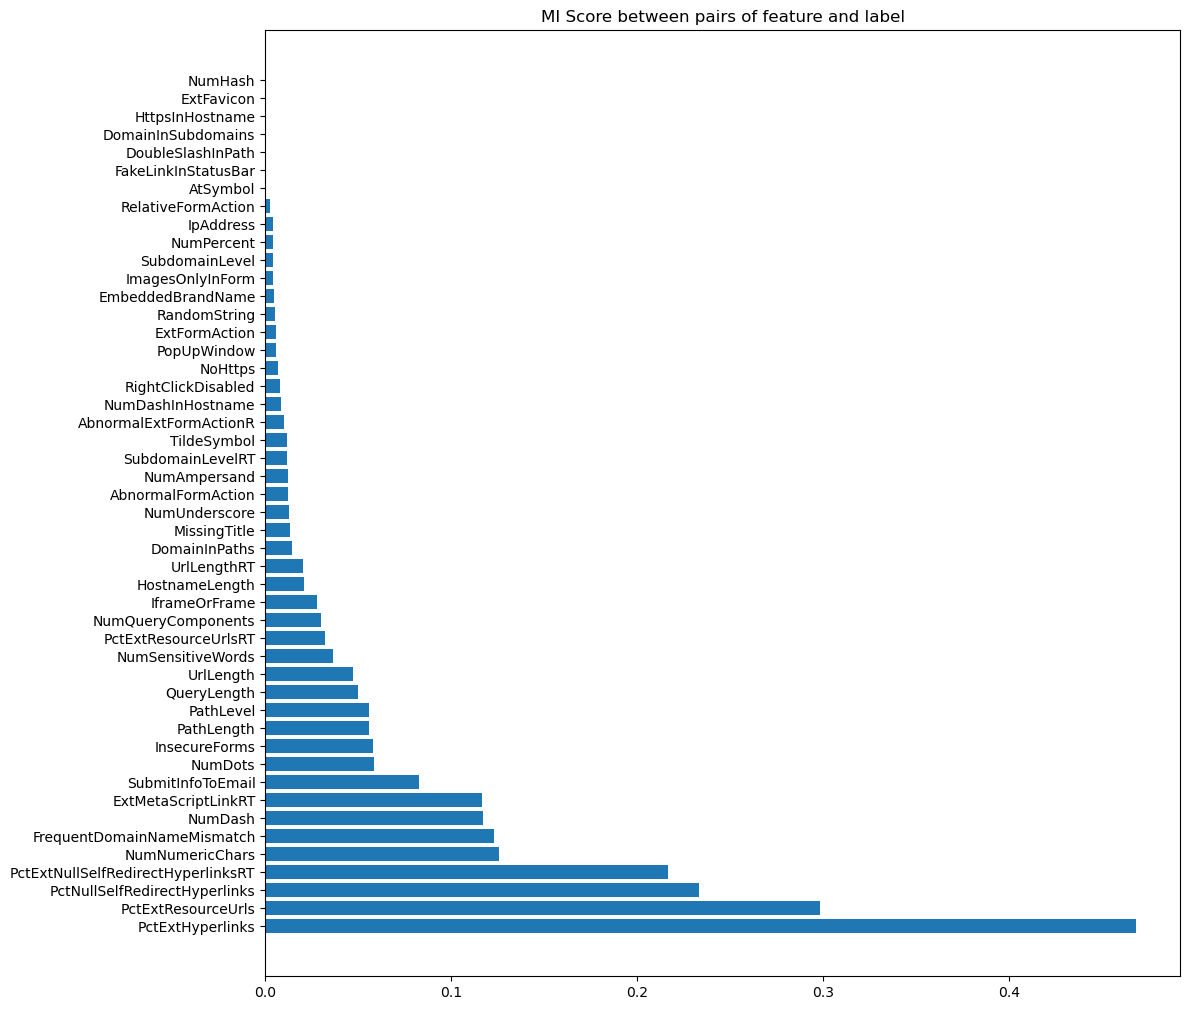
\includegraphics[width=\textwidth,height=\textheight,keepaspectratio,scale=1.5]
    {MI_score.png}
    \caption{Mutual Information (MI) Scores of all features}\label{fig:mi_score}
\end{figure}
\end{appendix}

\end{document}